\documentclass[a4paper,12pt,twoside]{memoir}

% Castellano
\usepackage[spanish,es-tabla]{babel}
\selectlanguage{spanish}
\usepackage[utf8]{inputenc}
\usepackage[T1]{fontenc}
\usepackage{lmodern} % Scalable font
\usepackage{microtype}
\usepackage{placeins}

\RequirePackage{booktabs}
\RequirePackage[table]{xcolor}
\RequirePackage{xtab}
\RequirePackage{multirow}

% Links
\usepackage[colorlinks]{hyperref}
\hypersetup{
	allcolors = {red}
}

% Ecuaciones
\usepackage{amsmath}

% Rutas de fichero / paquete
\newcommand{\ruta}[1]{{\sffamily #1}}

% Párrafos
\nonzeroparskip


% Imagenes
\usepackage{graphicx}
\newcommand{\imagen}[2]{
	\begin{figure}[!h]
		\centering
		\includegraphics[width=0.9\textwidth]{#1}
		\caption{#2}\label{fig:#1}
	\end{figure}
	\FloatBarrier
}

\newcommand{\imagenflotante}[2]{
	\begin{figure}%[!h]
		\centering
		\includegraphics[width=0.9\textwidth]{#1}
		\caption{#2}\label{fig:#1}
	\end{figure}
}



% El comando \figura nos permite insertar figuras comodamente, y utilizando
% siempre el mismo formato. Los parametros son:
% 1 -> Porcentaje del ancho de página que ocupará la figura (de 0 a 1)
% 2 --> Fichero de la imagen
% 3 --> Texto a pie de imagen
% 4 --> Etiqueta (label) para referencias
% 5 --> Opciones que queramos pasarle al \includegraphics
% 6 --> Opciones de posicionamiento a pasarle a \begin{figure}
\newcommand{\figuraConPosicion}[6]{%
  \setlength{\anchoFloat}{#1\textwidth}%
  \addtolength{\anchoFloat}{-4\fboxsep}%
  \setlength{\anchoFigura}{\anchoFloat}%
  \begin{figure}[#6]
    \begin{center}%
      \Ovalbox{%
        \begin{minipage}{\anchoFloat}%
          \begin{center}%
            \includegraphics[width=\anchoFigura,#5]{#2}%
            \caption{#3}%
            \label{#4}%
          \end{center}%
        \end{minipage}
      }%
    \end{center}%
  \end{figure}%
}


%
% Comando para incluir imágenes en formato apaisado (sin marco).
\newcommand{\figuraApaisadaSinMarco}[5]{%
  \begin{figure}%
    \begin{center}%
    \includegraphics[angle=90,height=#1\textheight,#5]{#2}%
    \caption{#3}%
    \label{#4}%
    \end{center}%
  \end{figure}%
}
% Para las tablas
\newcommand{\otoprule}{\midrule [\heavyrulewidth]}
%
% Nuevo comando para tablas pequeñas (menos de una página).
\newcommand{\tablaSmall}[5]{%
 \begin{table}
  \begin{center}
   \rowcolors {2}{gray!35}{}
   \begin{tabular}{#2}
    \toprule
    #4
    \otoprule
    #5
    \bottomrule
   \end{tabular}
   \caption{#1}
   \label{tabla:#3}
  \end{center}
 \end{table}
}

%
% Nuevo comando para tablas pequeñas (menos de una página).
\newcommand{\tablaSmallSinColores}[5]{%
 \begin{table}[H]
  \begin{center}
   \begin{tabular}{#2}
    \toprule
    #4
    \otoprule
    #5
    \bottomrule
   \end{tabular}
   \caption{#1}
   \label{tabla:#3}
  \end{center}
 \end{table}
}

\newcommand{\tablaApaisadaSmall}[5]{%
\begin{landscape}
  \begin{table}
   \begin{center}
    \rowcolors {2}{gray!35}{}
    \begin{tabular}{#2}
     \toprule
     #4
     \otoprule
     #5
     \bottomrule
    \end{tabular}
    \caption{#1}
    \label{tabla:#3}
   \end{center}
  \end{table}
\end{landscape}
}

%
% Nuevo comando para tablas grandes con cabecera y filas alternas coloreadas en gris.
\newcommand{\tabla}[6]{%
  \begin{center}
    \tablefirsthead{
      \toprule
      #5
      \otoprule
    }
    \tablehead{
      \multicolumn{#3}{l}{\small\sl continúa desde la página anterior}\\
      \toprule
      #5
      \otoprule
    }
    \tabletail{
      \hline
      \multicolumn{#3}{r}{\small\sl continúa en la página siguiente}\\
    }
    \tablelasttail{
      \hline
    }
    \bottomcaption{#1}
    \rowcolors {2}{gray!35}{}
    \begin{xtabular}{#2}
      #6
      \bottomrule
    \end{xtabular}
    \label{tabla:#4}
  \end{center}
}

%
% Nuevo comando para tablas grandes con cabecera.
\newcommand{\tablaSinColores}[6]{%
  \begin{center}
    \tablefirsthead{
      \toprule
      #5
      \otoprule
    }
    \tablehead{
      \multicolumn{#3}{l}{\small\sl continúa desde la página anterior}\\
      \toprule
      #5
      \otoprule
    }
    \tabletail{
      \hline
      \multicolumn{#3}{r}{\small\sl continúa en la página siguiente}\\
    }
    \tablelasttail{
      \hline
    }
    \bottomcaption{#1}
    \begin{xtabular}{#2}
      #6
      \bottomrule
    \end{xtabular}
    \label{tabla:#4}
  \end{center}
}

%
% Nuevo comando para tablas grandes sin cabecera.
\newcommand{\tablaSinCabecera}[5]{%
  \begin{center}
    \tablefirsthead{
      \toprule
    }
    \tablehead{
      \multicolumn{#3}{l}{\small\sl continúa desde la página anterior}\\
      \hline
    }
    \tabletail{
      \hline
      \multicolumn{#3}{r}{\small\sl continúa en la página siguiente}\\
    }
    \tablelasttail{
      \hline
    }
    \bottomcaption{#1}
  \begin{xtabular}{#2}
    #5
   \bottomrule
  \end{xtabular}
  \label{tabla:#4}
  \end{center}
}



\definecolor{cgoLight}{HTML}{EEEEEE}
\definecolor{cgoExtralight}{HTML}{FFFFFF}

%
% Nuevo comando para tablas grandes sin cabecera.
\newcommand{\tablaSinCabeceraConBandas}[5]{%
  \begin{center}
    \tablefirsthead{
      \toprule
    }
    \tablehead{
      \multicolumn{#3}{l}{\small\sl continúa desde la página anterior}\\
      \hline
    }
    \tabletail{
      \hline
      \multicolumn{#3}{r}{\small\sl continúa en la página siguiente}\\
    }
    \tablelasttail{
      \hline
    }
    \bottomcaption{#1}
    \rowcolors[]{1}{cgoExtralight}{cgoLight}

  \begin{xtabular}{#2}
    #5
   \bottomrule
  \end{xtabular}
  \label{tabla:#4}
  \end{center}
}


















\graphicspath{ {./img/} }

% Capítulos
\chapterstyle{bianchi}
\newcommand{\capitulo}[2]{
	\setcounter{chapter}{#1}
	\setcounter{section}{0}
	\chapter*{#2}
	\addcontentsline{toc}{chapter}{#2}
	\markboth{#2}{#2}
}

% Apéndices
\renewcommand{\appendixname}{Apéndice}
\renewcommand*\cftappendixname{\appendixname}

\newcommand{\apendice}[1]{
	%\renewcommand{\thechapter}{A}
	\chapter{#1}
}

\renewcommand*\cftappendixname{\appendixname\ }

% Formato de portada
\makeatletter
\usepackage{xcolor}
\newcommand{\tutor}[1]{\def\@tutor{#1}}
\newcommand{\course}[1]{\def\@course{#1}}
\definecolor{cpardoBox}{HTML}{E6E6FF}
\def\maketitle{
  \null
  \thispagestyle{empty}
  % Cabecera ----------------
\noindent
\includegraphics[width=\textwidth]{cabecera}\vspace{1cm}%
  \vfill
  % Título proyecto y escudo informática ----------------
  \colorbox{cpardoBox}{%
    \begin{minipage}{.8\textwidth}
      \vspace{.5cm}\Large
      \begin{center}
      \textbf{TFG del Grado en Ingeniería Informática}\vspace{.6cm}\\
      \textbf{\LARGE\@title{}}
      \end{center}
      \vspace{.2cm}
    \end{minipage}

  }%
  \hfill\begin{minipage}{.20\textwidth}
    
\includegraphics[width=\textwidth]{escudoInfor}
  \end{minipage}
  \vfill
  % Datos de alumno, curso y tutores ------------------
  \begin{center}%
  {%
    \noindent\LARGE
    Presentado por \@author{}\\ 
    en Universidad de Burgos --- \@date{}\\
    Tutores: \@tutor{}\\
  }%
  \end{center}%
  \null
  \cleardoublepage
  }
\makeatother

\newcommand{\nombre}{Adrián Antón García} %%% cambio de comando

% Datos de portada
\title{UBUSETAS}
\author{\nombre}
\tutor{\\D. José F. Díez Pastor \\D. Raúl Marticorena Sánchez}
\date{\today}

\begin{document}

\maketitle


\newpage\null\thispagestyle{empty}\newpage


%%%%%%%%%%%%%%%%%%%%%%%%%%%%%%%%%%%%%%%%%%%%%%%%%%%%%%%%%%%%%%%%%%%%%%%%%%%%%%%%%%%%%%%%
\thispagestyle{empty}


\noindent
\includegraphics[width=\textwidth]{cabecera}\vspace{1cm}

\noindent D. nombre tutor, profesor del departamento de nombre departamento, área de nombre área.

\noindent Expone:

\noindent Que el alumno D. \nombre, con DNI dni, ha realizado el Trabajo final de Grado en Ingeniería Informática titulado título de TFG. 

\noindent Y que dicho trabajo ha sido realizado por el alumno bajo la dirección del que suscribe, en virtud de lo cual se autoriza su presentación y defensa.

\begin{center} %\large
En Burgos, {\large \today}
\end{center}

\vfill\vfill\vfill

% Author and supervisor
\begin{minipage}{0.45\textwidth}
\begin{flushleft} %\large
Vº. Bº. del Tutor:\\[2cm]
D. nombre tutor
\end{flushleft}
\end{minipage}
\hfill
\begin{minipage}{0.45\textwidth}
\begin{flushleft} %\large
Vº. Bº. del co-tutor:\\[2cm]
D. nombre co-tutor
\end{flushleft}
\end{minipage}
\hfill

\vfill

% para casos con solo un tutor comentar lo anterior
% y descomentar lo siguiente
%Vº. Bº. del Tutor:\\[2cm]
%D. nombre tutor


\newpage\null\thispagestyle{empty}\newpage




\frontmatter

% Abstract en castellano
\renewcommand*\abstractname{Resumen}
\begin{abstract}
Proyecto en el que se va a desarrollar una aplicación Android que permita mediante la fotografía de una seta clasificar a que especie pertenece. Además se proporcionará información de las especies más probables, así como imágenes de estas especies para comparar con nuestra fotografía.

Para realizar la parte del reconocimiento de imágenes se aplicarán técnicas de minería de datos para usar los clasificadores de imágenes.

A la hora de recopilar la información necesaria, se usarán técnicas de Web semántica para conseguir una pequeña descripción e información interesante sobre cada especie de seta. Esta parte se realizará realizando consultas a la DBpedia.

Para completar el trabajo del clasificador de imágenes, se integrarán diferentes claves dicotómicas para el reconocimiento de géneros y especies de setas. Estas claves se conseguirán realizando técnicas de Web Scraping.

El objetivo del proyecto es el de crear una herramienta que sirva de apoyo en las tareas de Micología relacionadas con el reconocimiento de setas.
\end{abstract}

\renewcommand*\abstractname{Descriptores}
\begin{abstract}
\textbf{Palabras clave.} \textit{Minería de datos, Clasificador, Web Semántica, Clave dicotómica, Android, Seta, Micología, Reconocimiento}
\end{abstract}

\clearpage

% Abstract en inglés
\renewcommand*\abstractname{Abstract}
\begin{abstract}
Project in which you can develop an Android application that allows by photographing a mushroom to classify the species it belongs to. You can also get information on the most likely species, as well as images of these species to compare with our photograph.

To perform the image recognition part, data mining techniques are used to use the image classifiers.

When compiling the necessary information, use semantic Web techniques to get a short description and interesting information about each species of mushroom. This part refers to DBpedia queries.

To complete the work of the image classifier, the different dichotomous keys are integrated for the recognition of the genera and species of the mushrooms. These keys were obtained by performing Web Scraping techniques.

The objective of the project is to create a tool that will support the Mycology tasks related to the recognition of mushrooms.
\end{abstract}

\renewcommand*\abstractname{Keywords}
\begin{abstract}
\textbf{Keywords} \textit{Data Mining, Sorter, Semantic Web, Dichotomous Key, Android, Mushroom, Mycology, Recognition}
\end{abstract}

\clearpage

% Indices
\tableofcontents

\clearpage

\listoffigures

\clearpage

\listoftables
\clearpage

\mainmatter
\capitulo{1}{Introducción}

La tarea de clasificar una seta es altamente compleja ya que las diferencias entre algunas especies son mínimas y se necesitan de expertos que las analicen detalladamente hasta clasificar con seguridad la especie. Además dependiendo de la fase de crecimiento en la que se encuentre la propia seta y los factores a los que se encuentre expuesta, como puede ser la humedad del ambiente, pueden provocar que la apariencia de la seta cambie dificultando aún más esta tarea. 

La clasificación de una seta debe realizarse de forma segura y minuciosa ya que hay que asegurarse que la seta no sea tóxica ni provoque perjuicios a aquella persona que la consuma.

Ante estas dificultades nace la idea de crear una aplicación que nos ayude con la identificación de la especie o género a la que pertenece una seta. Debe quedar claro desde el principio que esta aplicación solo debe servir de guía y no pretende sustituir los conocimientos de un experto, simplemente servir de apoyo o de ayuda en la difícil tarea de clasificar la especie a la que pertenece una seta. 

Por estos motivos los resultados obtenidos por el clasificador deben tomarse sólo como una ayuda y usarlos para encaminar nuestra búsqueda de la especie correcta en el buen camino.

Para hacer uso de la aplicación, deberemos introducir una foto de la seta a clasificar, bien directamente sacando una foto desde la cámara o desde la galería de nuestro móvil. Con esta foto la aplicación nos mostrará las especies que el clasificador ha determinado como más probables. Si pulsamos sobre cada especie mostrada se nos mostrará información de esa especie, una breve descripción, la comestibilidad, así como diferentes imágenes que podremos comparar con la seta a clasificar. Además de mostrar esta información, la aplicación nos hará preguntas mediante claves dicotómicas según los resultados obtenidos para identificar correctamente la seta. Las preguntas consistirán en una breve descripción de características de la seta, el usuario deberá elegir la que más se adecue a la seta para poder llegar a la especie concreta.

La aplicación se ejecuta íntegramente en el móvil, es decir, no necesitaremos de una conexión a Internet para ejecutar el clasificador ni obtener información de la seta. Actualmente el clasificador es capaz de ejecutarse en el propio móvil sin necesidad de un servidor externo en un tiempo casi instantáneo permitiendo diferenciar entre 173 especies de setas diferentes. La aplicación cuenta con una pequeña base de datos que contiene información de cada especie, si lo deseamos podemos acceder por Internet al link proporcionado en cada especie a la página en la Wikipedia de la especie.
\capitulo{2}{Objetivos del proyecto}
%Este apartado explica de forma precisa y concisa cuales son los objetivos que se persiguen con la realización del proyecto. Se puede distinguir entre los objetivos marcados por los requisitos del software a construir y los objetivos de carácter técnico que plantea a la hora de llevar a la práctica el proyecto.

En este apartado se va a proceder a explicar los objetivos marcados en el proyecto, diferenciando entre los objetivos generales que se requerían para llevar a cabo este proyecto y los objetivos técnicos que se han ido encontrando a lo largo de su ejecucción.

\section{Objetivos Generales}

A continuación se muestran los principales objetivos del proyecto de forma general:

\begin{itemize}
	\item El objetivo principal del proyecto es el de crear una aplicación Android que fuera capaz de identificar, mediante un clasificador de imágenes, la especie a la que pertenece una seta mediante una fotografía introducida por el usuario, bien por la cámara o desde la galería del móvil.
	\item Otro objetivo es el de mostrar información de las diferentes especies clasificadas. En esta información se incorporaría una breve descripción de la especie, la comestibilidad y otros datos de interés. Este objetivo se realizará mediante técnicas de web semántica.
	\item Como complemento al clasificador se debería implementar una serie de claves dicotómicas que mediante preguntas simples acerca de la seta conduzcan a la especie correcta de la que se trata. Este objetivo se implementará mediante técnicas de web scraping.
	\item Se intentará desarrollar una interfaz atractiva y amigable en la aplicación Android.
\end{itemize}

\section{Objetivos Técnicos}

En esta lista se van a detallar los objetivos técnicos que se han planteado para implementar los objetivos generales descritos anteriormente.

\begin{itemize}
	\item Usar Android Studio para implementar la aplicación Android.
	\item Un objetivo técnico importante que se marcó fue el de ejecutar el clasificador en el propio móvil, para lo que se utilizaron las librerías de Tensorflow para Android Studio junto a los modelos de clasificación Mobilenet.
	\item Usar Java como lenguaje de programación principal a la hora de programar la parte de Web Semántica y la extracción de las claves dicotómicas mediante Web Scraping.
	\item Utilizar Sparql como lenguaje para realizar las consultas a la DBpedia.
	\item Usar las librerías de Apache Jena para realizar las consultas con sparql a la DBpedia en Java y extraer la información de las especies de setas.
	\item Utilizar las librerías de Jaunt en java para realizar la parte de Web Scraping y poder extraer las claves dicotómicas.
	\item Utilizar SQlite como base de datos para almacenar los datos de las especies y las claves en Android.
	\item Usar un sistema de control de versiones, se ha optado por utilizar el servicio GitHub.
	\item Utilizar la metodología Scrum para realizar un seguimiento de las tareas realizadas durante el proyecto. Se ha elegido usar la herramienta ZenHub para este propósito.
	\item Se intentará que la aplicación no ocupe demasiada memoria dentro del dispositivo, para ello se formatearán las imágenes para que ocupen lo necesario y se buscará un modelo de clasificador que no sea demasiado exigente, en nuestro caso se ha optado por el modelo Mobilenet-224-v1.
	\item Llevar a cabo un prototipo de la interfaz de usuario mediante alguna herramienta de prototipado.
	\item Utilizar herramientas de testing para probar el correcto funcionamiento de nuestra aplicación.
	\item Hacer uso de las directrices de diseño de Material design para desarrollar la interfaz gráfica.
\end{itemize}

\capitulo{3}{Conceptos teóricos}

Para la correcta comprensión del proyecto se van a explicar a continuación una serie de conceptos teóricos mínimos necesarios.

\section{Micología}

La micología es la ciencia que se dedica al estudio de los hongos. Es una de las áreas de la ciencia más extensas y diversificadas que aporta avances significativos a la investigación científica y al desarrollo tecnológico \cite{wiki:micologia}.

Tiene varios aplicaciones y objetivos, se usa para determinar que especies de hongos son comestibles o no y si podrían usarse para diferentes tratamientos médicos, ciertas sustancias de las setas son estudiadas con estos fines curativos \cite{micologiaDef}. 

\section{Hongos}

El hongo es el nombre común de los organismos del reino Fungi. El término Fungi en biología se refiere a un grupo de organismos eucariotas\footnote{Aquellos organismos formados por células con núcleo verdadero} que se clasifican en un reino distinto al de las plantas, animales y protistas. Se diferencian de las plantas en que son heterótrofos\footnote{Seres vivos que necesitan de otros para alimentarse} y de los animales en que tienen paredes celulares, como las plantas, pero compuestas de quitina\footnote{\url{https://es.wikipedia.org/wiki/Quitina}} en vez de celulosa.

Los hongos se reproducen de forma sexual o asexual mediante esporas, que se dispersan en un estado latente y solo se interrumpe cuando se dan las condiciones adecuadas para su germinación \cite{wiki:fungi}. 

La mayoría de los hongos están formados por estructuras microscópicas, filamentosas y ramificadas llamadas hifas. El conjunto de estas hifas forma una red a la que llamaremos micelio. Cuando la acumulación de hifas es grande se pueden observar como una red algonodosa que se pueden reconocer por ejemplo cuando los alimentos empiezan a descomponerse \cite{setas}.

\section{Setas}

Las setas son los cuerpos fructíferos de algunos tipos de hongos (no todos los hongos producen setas), en otras palabras, son la parte reproductiva de los hongos. La principal función de la seta es dispersar las esporas del hongo. Normalmente es la parte visible del hongo ya que este suele estar bajo tierra.

\subsection{Partes de las setas}

A continuación se van a describir las partes más características de una seta que se usan para su clasificación.

\begin{itemize}
	\item{Sombrero}: Situado sobre el pie, ejerce la función de protección en la formación y desarrollo de las esporas. El sombrero es un elemento clave a la hora de diferenciar las especies ya que puede adoptar diferentes formas, aspectos y colores.
	\item{Himenio}: Es la parte situada justo debajo del sobrero y que puede adoptar diferentes formas (láminas, tubos, aguijones o pliegues), estas diferentes formas nos ayudarán a diferenciar entre las especies. La función principal de esta parte es la de crear, desarrollar, almacenar y dispersar las esporas que generan nuevos hongos.
	\item{Lamina}: Son los tabiques del himenio que contienen los basidios\footnote{Estructuras microscópicas que generan las esporas de la seta}.
	\item{Pie}: Elemento que no tiene por que aparecer en todas las setas y que sujeta al sombrero e himenio.
	\item{Volva}: Es un fragmento en forma de membrana que envuelve la base del pie en algunas setas. Es un error común cortar el pie de la seta y no conservar la volva que nos podría dar indicios de a qué especie pertenece la seta.
	\item{Micelio}: El conjunto de hifas, es decir, el hongo propiamente dicho \cite{partesSeta}.
\end{itemize}

%http://www.fungiturismo.com/todas-partes-de-seta

En la siguiente figura \ref{figpartesDeLaSeta} se muestran las partes más relevantes de una seta.

\begin{figure}[h]
    \begin{center}%
        \begin{center}%
          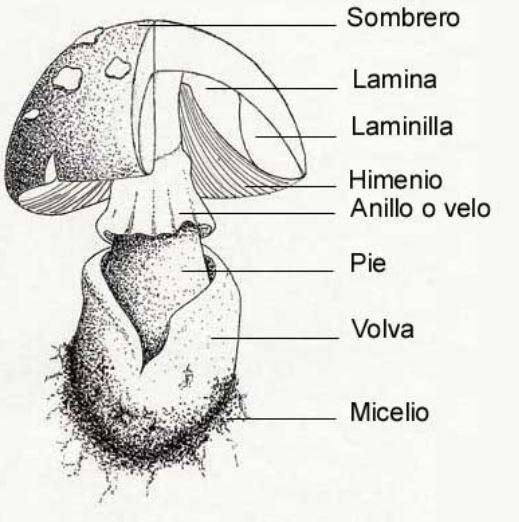
\includegraphics[width=1\textwidth]{partesDeLaSeta}%
          \caption{Partes de una seta \cite{imagenPartesSeta}}%
          \label{figpartesDeLaSeta}%
        \end{center}%
  	\end{center}%
\end{figure}%

\newpage
%https://lameleracasarural.files.wordpress.com/2014/11/partesdelaseta.jpg
\section{Inteligencia Artificial}
%https://luismejias21.files.wordpress.com/2017/09/inteligencia-artificial-un-enfoque-moderno-stuart-j-russell.pdf
Hay muchas definiciones para definir lo que es la inteligencia artificial, normalmente aparece bajo las siglas IA o AI (del inglés Artificial Intelligence), pero de forma general la podemos definir como el desarrollo de algoritmos y métodos que otorgan a las computadoras la capacidad de realizar acciones o tareas como las realizaría un ser humano. La inteligencia artificial se aplica en multitud de campos como puede ser la robótica, automovilismo, reconocimiento de imágenes, medicina, sistemas de apoyo...

Stuart Russell y Peter Norving \cite{wiki:tiposInteligenciaArtificial}  diferencian estos cuatro tipos de inteligencia artificial:

\begin{itemize}
	\item{Sistemas que piensan como humanos}: Son sistemas que intentan emular el pensamiento humano automatizando actividades que relacionamos con los procesos de pensamiento humano (toma de decisiones, resolución de problemas...), por ejemplo las redes neuronales artificiales, usadas en los clasificadores de imágenes entrenados en este proyecto.
	\item{Sistemas que actúan como humanos}: Este tipo de sistemas intentan imitar el comportamiento humano, por ejemplo la robótica.
	\item{Sistemas que piensan racionalmente}: Tratan de imitar con lógica el pensamiento lógico racional del ser humano, por ejemplo los sistemas expertos.
	\item{Sistemas que actúan racionalmente}: Intentan emular de forma racional el comportamiento humano.
\end{itemize}

Algunos de estos sistemas necesitan desarrollar una capacidad de aprendizaje para poder imitar de forma correcta el comportamiento humano.

\subsection{Aprendizaje automático}

El aprendizaje automático (del inglés Machine Learning) es una rama de la inteligencia artificial que se encarga de desarrollar los algoritmos que permitan a las computadoras aprender\footnote{Adquirir conocimiento por medio de la experiencia}. Para ello, se entrenan los sistemas con una serie de ejemplos, o información de entrenamiento, para generalizar comportamientos que deben realizar ante diferentes casos de entrada.

Hay una gran variedad de algoritmos de aprendizaje automático, a continuación se presentan algunos de los tipos más extendidos:
\begin{itemize}

	\item{Aprendizaje supervisado}: en estos algoritmos se intenta crear una función que nos dé la correspondencia entre los datos de entrada y una de las salidas deseadas. En este tipo de algoritmos se tiene información tanto de los valores de entrada como del los valores deseados.Para entrenar se suelen usar pares en los que un componente son los datos de entrada y otro los valores deseados. Los valores deseados suelen ser denominados como clases \cite{wiki:aprendizaheSupervisado}.
	
	El valor de salida de la función puede ser un número (Regresión) o una etiqueta de clase (Clasificación).
	
	Los algoritmos de clasificación usados en este proyecto se corresponderían con este tipo de aprendizaje, siendo las etiquetas de clase las especies de setas que se quieren clasificar.
	
	\item{Aprendizaje no supervisado}: el aprendizaje no supervisado se diferencia del supervisado en que no se conoce a priori los resultados deseados. En este tipo de aprendizaje, normalmente, se tratan los datos de entrada como una serie de datos aleatorios y se intentan buscar relaciones ocultas entre ellos.
	Una forma de aprendizaje no supervisado es el clustering, el cuál se encarga de organizar los datos de entrada en grupos en los que comparten propiedades y los diferencian del resto \cite{wiki:aprendizajeNoSupervisado}.
	Un ejemplo de uso de este tipo de aprendizaje lo podemos encontrar en el proyecto \textit{IberoSetas 2.0} \cite{iberosetas}, en el que se usaba la técnica \textit{Bag of words} que usaba clustering. En este proyecto no se han necesitado usar este tipo de técnicas.
	
	\item{Aprendizaje semisupervisado}: Este tipo de aprendizaje mezcla las dos técnicas descritas anteriormente. Se usa cuando tenemos tanto datos conocidos como datos de los que no tenemos conocimiento.
	
	\item{Aprendizaje por refuerzo}: Este tipo de algoritmos realiza una aprendizaje mediante el modelo de prueba-error, es decir, el algoritmo realiza acciones y a partir de los resultados de estas el algoritmo evalúa cuáles han sido beneficiosas y cuáles no.
\end{itemize}
	
En nuestro proyecto se hace uso del aprendizaje supervisado para entrenar el clasificador de imágenes que reconocerá las especies de las setas \cite{wiki:aprendizajeAutomatico}.

\section{Minería de datos}

La minería de datos consiste en la aplicación de técnicas de inteligencia artificial sobre grandes cantidades de datos con el objetivo de descubrir patrones o relaciones ocultas entre los datos. La parte de la minería de datos más relevante para nuestro proyecto son los clasificadores previamente introducidos \cite{procesosMineriaDatos}. Básicamente los clasificadores se basan en la hipótesis del aprendizaje inductivo:

Cualquier hipótesis que aproxime bien una función objetivo sobre un conjunto de ejemplos de entrenamiento suficientemente grande también aproximará bien la función objetivo en ejemplos no observados,

La míneria de datos, típicamente, consta de los siguientes pasos:
\begin{itemize}
	\item{Selección del conjunto de datos}: En esta parte del proceso se seleccionarán las variables objetivo, las variables independientes y se realizará un muestreo con los registros disponibles.
	\item{Análisis de las propiedades de los datos}: Se comprobarán los histogramas, diagramas de dispersión, si se encuentran valores atípicos entre el conjunto de datos y si faltan ciertos datos.
	\item{Transformación de los datos}: En esta etapa del proceso se procesarán los datos de entrada para adecuarlos a la estructura requerida por las técnicas de inteligencia artificial que se aplicarán sobre ellos.
	\item{Selección de la técnica de minería de datos}: Se construirá el modelo predictivo a aplicar sobre los datos. Clasificación o segmentación.
	\item{Extracción del conocimiento}: Esta es la parte donde se aplicarán las técnicas de inteligencia artificial sobre los datos para extraer el conocimiento buscado. La técnica que hayamos aplicado nos devolverá un modelo de conocimiento sobre los datos.
	\item{Interpretación y evaluación de los datos}: Esta última etapa consiste en validar si los resultados que nos ofrece el modelo entrenado son satisfactorios y se adecuan a los requisitos pedidos.
\end{itemize}

\subsection{Evolución del flujo de trabajo}

Al principio, el flujo de trabajo para entrenar un clasificador, era el de extraer unas características de los datos de entrenamiento que se proporcionaban al clasificador. En este modo de trabajo se usan métodos como el Bag-of-words\footnote{Por ejemplo, tratar las características de una imágen como palabras y guardar las veces que se repiten estas características en cada imagen. \url{https://es.wikipedia.org/wiki/Modelo_bolsa_de_palabras}} para determinar las características de los datos de entrada \cite{iberosetas}.

Posteriormente, este flujo de trabajo se ha modificado, introduciendo redes neuronales que se encargan de extraer estas características y dividiéndolas en diferentes jerarquías para que no todas tengan el mismo peso a la hora de clasificar.

\begin{figure}[h]
    \begin{center}%
        \begin{center}%
          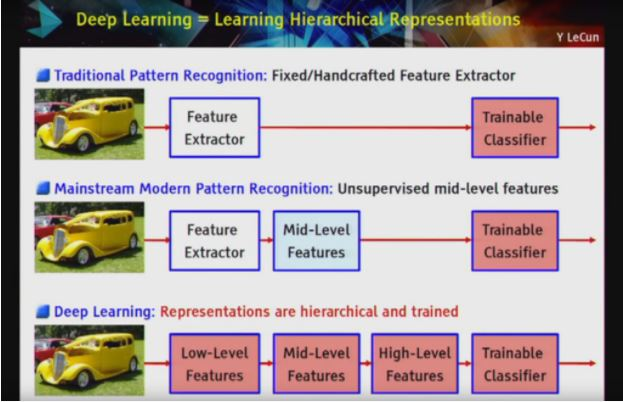
\includegraphics[width=0.7\textwidth]{FlujoTrabajo}%
          \caption{Flujos de trabajo, clasificación}%
          \label{figFlujo}%
        \end{center}%
  	\end{center}%
\end{figure}%

En la figura \ref{figFlujo} se muestra como se han ido incorporando diferentes capas, todas de ellas entrenables, para extraer las características de una forma jerárquica mediante redes neuronales  \cite{flujosTrabajo}.

\newpage

\section{Redes neuronales}

En esta sección se explicarán algunos conceptos teóricos sobre redes neuronales necesarios para entender el funcionamiento de los modelos Mobilenet e Inception usados para clasificar imágenes en nuestro proyecto. Actualmente hay gran variedad de clasificadores que se pueden usar para esta tarea además de los dos mencionados.

\subsection{Modelo de neurona artificial}

Una neurona artificial de forma general se puede describir según el modelo de Rumelhart y McClelland (1986), el cual define la neurona o elemento de proceso (EP) como un dispostivo el cuál a partir de un conjunto de entradas, vector x, genera una única salida y \cite{redesNeurnalesUno}. 

\begin{figure}[h]
    \begin{center}%
        \begin{center}%
          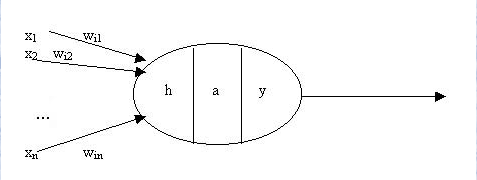
\includegraphics[width=1\textwidth]{modeloNeuronaArtificial}%
          \caption{Modelo de una neurona artificial}%
          \label{figmodeloNeuronaArtificial}%
        \end{center}%
  	\end{center}%
\end{figure}%

\newpage
La neurona artificial consta de los siguientes elementos:

\begin{itemize}
	\item{Conjunto de entradas x}: El vector x.
	\item{Conjunto de pesos sinápticos $w_{i,j}$ }: Representan la relación entre la neurona i y j.
	\item{Regla de propagación}: proporciona el potencial postsináptico, $h_i (t)$. Se suele representar como una suma ponderada de la siguiente forma \ref{eq:funcionPropagacion}
	
\begin{equation} \label{eq:funcionPropagacion}
	h_{1}(t)=\sum (w_{1j}*x_{j})
\end{equation}

	\item{Función de activación a}: proporciona el estado de activación en función del estado anterior y el potencial postsináptico.
	\item{Función de salida y}: proporciona la salida y en función del valor de activación. En la figura \ref{figfuncionesActivacion} podemos ver diferentes funciones de activación.
\end{itemize}

\begin{figure}[h]
    \begin{center}%
        \begin{center}%
          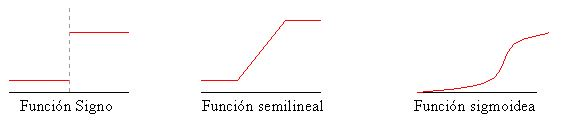
\includegraphics[width=1\textwidth]{funcionesActivacion}%
          \caption{Funciones de activación}%
          \label{figfuncionesActivacion}%
        \end{center}%
  	\end{center}%
\end{figure}%
\newpage

\subsection{Red Neuronal Artificial RNA}

Una red neuronal Artificial RNA es un grafo dirigido en el que las neuronas artificiales estas conectadas con otras y los enlaces pueden aumentar o disminuir el estado de activación de las neuronas conectadas. Cada neurona opera de forma individual mediante operaciones de suma \cite{wiki:redesNeuronalesArtificiales}.

Estas neuronas se organizan en capas o layers formando diferentes filtros para generar algoritmos que puedan resolver diferentes problemas. Dentro de una misma capa las neuronas suelen ser del mismo tipo y podemos diferenciar de forma general 3 tipos distintos de capas:

\begin{itemize}
	\item{De entrada}: Reciben datos o señales externos del entorno.
	\item{De salida}: Proporcionan las respuestas de la red ante los estímulos recibidos por las capas de entrada.
	\item{Ocultas}: No interaccionan con el entorno, son nodos intermedios que ejecutan las operaciones internas de la red.
\end{itemize}

\begin{figure}[h]
    \begin{center}%
        \begin{center}%
          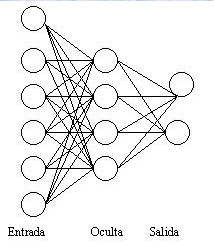
\includegraphics[width=0.7\textwidth]{RNA}%
          \caption{Grafo de una RNA}%
          \label{figRNA}%
        \end{center}%
  	\end{center}%
\end{figure}%

Como se puede observar en la figura \ref{figRNA}, las neuronas representadas como nodos se organizan en las diferentes capas pudiéndose interconectar con varias neuronas a la vez. Estas redes pueden tener un número de capas y neuronas ilimitados. Pueden tener un número ilimitado de enlaces o solo estar conectadas con unas pocas.

\newpage
\subsection{Redes neuronales convolucionales}

Este tipo de redes neuronales son muy parecidas a las RNA normales pero tienen dos cambios significativos. El primero es que parten de la idea de que las entradas son imágenes lo que permite programar optimizaciones a los algoritmos para que se adecuen a este tipo de entradas, el segundo cambio es que intentan reducir en la mayor medida posible el número de parametros utilizados en cada capa \cite{redesNeuronalesConvolucionales}.

\begin{figure}[h]
    \begin{center}%
        \begin{center}%
          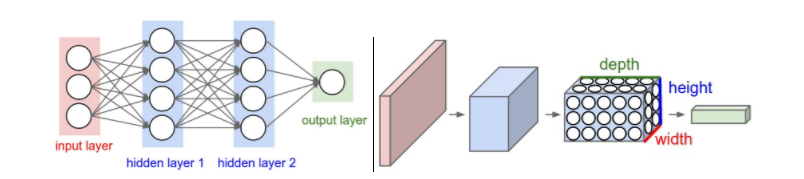
\includegraphics[width=1\textwidth]{RNAvsConvolucional}%
          \caption[Comparativa de grafos]{Izquierda: grafo de una RNA. Derecha: Grafo de una Red neuronal convolucional.}%
          \label{figRNAvsConvolucional}%
        \end{center}%
  	\end{center}%
\end{figure}%

Las redes neuronales convolucionales organizan sus neuronas en capas de 3 dimensiones normalmente coincidiendo con las características de la imagen, siendo \textit{height} la altura de la foto, \textit{width} el ancho y \textit{depth} los colores de la imagen. Por ejemplo se podría aplicar a imágenes de 32x32x3.

\subsection{Tipos de capas}

En este apartado se van a explicar los tres tipos de capas más importantes a la hora de elabora las redes neuronales convolucionales:
%https://ccc.inaoep.mx/~pgomez/deep/presentations/2016Loncomilla.pdf
\subsubsection{Capas convolucionales}

En estas capas los pixeles de salida son combinaciones lineales de diferentes pixeles de entrada lo que generan nuevos mapas de pixeles mas sencillos y que no son tan sensibles a cualquier cambio en los pixeñes de las entradas \cite{redesConvolucionales}. Las convoluciones se pueden producir teniendo en cuenta solo 2 dimensiones (el alto y ancho) o teniendo en cuenta las 3 dimensiones (alto, ancho y profundidad). Las capas convolucionales llamadas RELU ejecutan la función de activación de las neuronas.

\begin{figure}[h]
    \begin{center}%
        \begin{center}%
          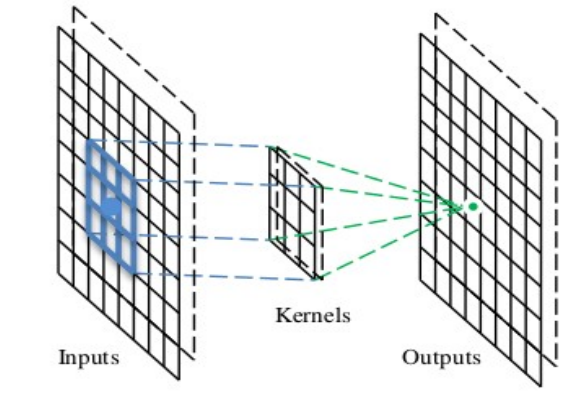
\includegraphics[width=0.7\textwidth]{convolucion}%
          \caption[Convolución de dos dimensiones]{Figura que muestra una convolución en dos dimensiones.}%
          \label{figconvolucion}%
        \end{center}%
  	\end{center}%
\end{figure}%
 
Como vemos en la figura \ref{figconvolucion} Los kernels definen el área sobre el que se va a aplicar la convolucion, en el ejemplo 3x3.

\subsubsection{Capas de pooling}

Las capas de pooling o reescalado tiene el objetivo de disminuir el número de parámetros o pixeles de los mapas, para ello se aplican técnicas como la explicada en la siguiente figura.

Estas capas van a tener un gran peso en los modelos de Mobilenet e Inception, ya que nos van a permitir ajustar el número de operaciones realizadas por los modelos para que se puedan ajustar correctamente a las limitaciones hardware de los teléfonos móviles.

\begin{figure}[h]
    \begin{center}%
        \begin{center}%
          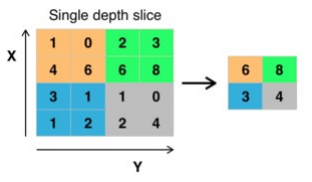
\includegraphics[width=0.7\textwidth]{pooling}%
          \caption{Técnica de máx pooling.}%
          \label{figpooling}%
        \end{center}%
  	\end{center}%
\end{figure}%

En la figura \ref{figpooling} se puede observar que los diferentes pixeles se agrupan eligiendo sólo aquellos de mayor valor para el nuevo mapa.

\subsubsection{Capas totalmente conectadas}

En este tipo de capas las neuronas están totalmente conectadas con las neuronas de la capa anterior y tienen una profundidad igual al número de clases que se quieran clasificar. Por ejemplo si tenemos 10 clases diferentes, el último layer podría ser de tamaño 32x32x10. Estas capas son las encargadas de producir la señal de salida y clasificar la imagen eligiendo una de las clases. 

Cuando re-entrenamos un modelo, normalmente lo que estamos haciendo es modificar estas últimas capas que se encargan de clasificar las clases en vez de tener que re entrenar todas las demás capas que forman el modelo.

\section{Modelo Inception}

El modelo Inception es una red neuronal convolucional que se usa para la clasificación de imagenes. Inception ha sido desarrollado por Google y parte de la pregunta de que tipo de convolución aplicar en cada capa o  filtro del modelo. Es decir, preguntarse que tamaño de convolución sería el adecuado para cada etapa, ¿3x3?,¿1x1?,¿5x5? \cite{depthwiseSeparableConvolutions}.

Ante esta pregunta, la respuesta que han aplicado es la de ejecutar los diferentes tamaños de convoluciones en cada capa de manera paralela y concatenar los diferentes mapas en uno solo que es el que se pasa a la siguiente capa del modelo. La idea es ejecutar todos los tipos de convulciones a la vez y elegir el que mejor funcione.

\begin{figure}[h]
    \begin{center}%
        \begin{center}%
          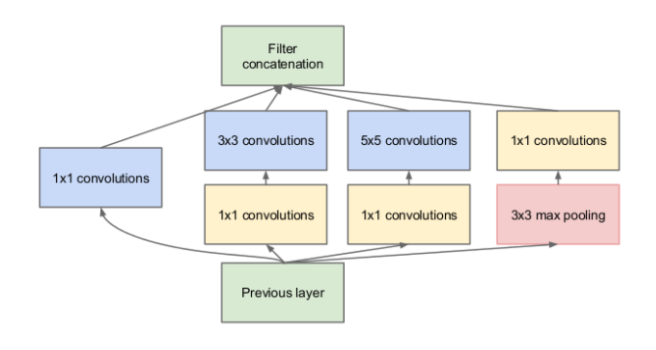
\includegraphics[width=1\textwidth]{inception}%
          \caption{Ejemplo de un nodo Inception.}%
          \label{figinception}%
        \end{center}%
  	\end{center}%
\end{figure}%

En la figura \ref{figinception} podemos observar como se aplican las diferentes convoluciones en pararelo. Además podemos observar que se aplican unas convoluciones de 1x1, estas convoluciones tienen el objetivo de reducir el número de parámetros que se usan ya que aunque no reducen el área de los mapas sí reducen la profundidad de las capas \cite{inception}.

Los modelos inception se construyen concatenando estos bloques o nodos Inception, en teoría cuanta más profundidad se dé a estos modelos y más se concatenen más precisos deberían ser los modelos pero esto tiene un coste alto de computación (Aún reduciendo los computos con las convoluciones 1x1) y se corre el riesgo de sobreajustar los modelos.

Actualmente se pueden entrenar diferentes versiones de Inception, en el proyecto hemos trabajado reentrenando la versión 3 del modelo mediante Tensorflow.

Este modelo se sigue desarrollando y los desarrolladores lo van evolucionando por lo que no es de extrañar que en un futuro cercano aparezcan nuevas versiones mas optimizadas de este modelo.

\begin{figure}[h]
    \begin{center}%
        \begin{center}%
          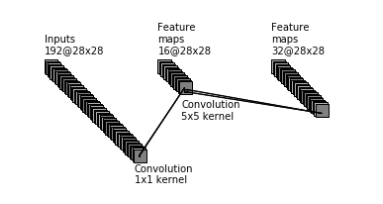
\includegraphics[width=1\textwidth]{convolicionReduccion}%
          \caption[Aplicación convoluciones]{Aplicación de una convolucion 1x1 antes de ejecutar la convolucion 5x5.}%
          \label{figconvolicionReduccion}%
        \end{center}%
  	\end{center}%
\end{figure}%

En la figura \ref{figconvolicionReduccion} se puede observar el efecto de aplicar una convolucion 1x1 antes de efectuar la convolucion 5x5.

\section{Modelo Mobilenet}

Mobilenet hace referencia a una serie de modelos clasificadores de imágenes desarrollados por Google para ser embebidos en dispositivos móviles o sistemas con pocos recursos. La filosofía de este tipo de clasificadores nace en contraposición a la tendencia que se estaba implantando en las redes neuronales de crear redes profundas y complejas con el objetivo de mejorar la precisión dejando a un lado cuestiones como el tamaño del modelo o la rapidez \cite{mobilenet}.

Los modelos Mobilenet intentan ser precisos pero a la vez ser modelos de poco tamaño y rápidos que se adecuen a sistemas que necesiten de estas ventajas, como pueden ser los automóviles autónomos, realidad aumentada, sistemas de reconocimiento, entre otros.

La arquitectura de este tipo de modelo, al igual que el modelo Inception explicado anteriormente, se basa en una red neuronal convolucional que se explicará en el siguiente apartado.

\subsection{Arquitectura Modelo Mobilenet}

La arquitectura del modelo Mobilenet se basa en dividir los filtros convolucionales típicos de una RNA totalmente conectada en dos nuevos tipos de filtros, los filtros convolucionales profundos (del inglés Depthwise Convolutional Filters) y los filtros convolucionales puntuales (del inglés Pointwise Convolution Filters).

El objetivo de esta división de fitros es el de minimizar el número de operaciones realizada. La convoluciones normales tienen el siguiente coste \ref{eq:convolucionNormal}:

\begin{equation} \label{eq:convolucionNormal}
	DK * DK * M * N * DF * DF
\end{equation}

DK=Tamaño del kernel (alto x ancho), M=Número de canales de entrada, N=número de canales de salida, DF=Tamaño del mapa de salida.

Los Depthwise Convolutional Filters tienen el siguiente coste computacional \ref{eq:convolutionalFilter}:

\begin{equation} \label{eq:convolutionalFilter}
	DK * DK * M * DF * DF
\end{equation}

Y los Pointwise Convolution Filters tienen el siguiente coste \ref{eq:pointwiseFilter};

\begin{equation} \label{eq:pointwiseFilter}
	M * N * DF * DF
\end{equation}

Si expresamos la convolución como un proceso de dos pasos de filtrado y combinación de los dos filtros anteriores obtenemos la siguiente reducción de costes de computación \ref{eq:convolución}:
\begin{equation} \label{eq:convolución}
\frac{(DK * DK * M * DF * DF + M * N * DF * DF)}{(DK * DK * M * N * DF * DF) }= (1/N)+(1/(DK*DK))
\end{equation}

Lo que supone una reducción respecto a los filtros convolucionales normales. Esta reducción la podemos observar en la siguiente tabla:
\newpage
\tablaSmall{Depthwise Separable vs Full Convolution MobileNet}{l c c c}{herramientasportipodeuso}
{ \multicolumn{1}{l}{Modelos} & Imagenet Accuracy & Million Mult-Adds & Million Parameters \\}{ 
Conv MobileNet & 71.7\% & 4866 & 29.3 \\
MobileNet & 70.6\% & 569 & 4.2 \\
} 

Estos dos tipos de filtros se aplican de forma separada y paralela como sucedía en el modelo Inception. Para ver como surgen estas convoluciones vamos a fijarnos en la siguiente figura \ref{figconvolucionesMobilenet}.

\begin{figure}[h]
    \begin{center}%
        \begin{center}%
          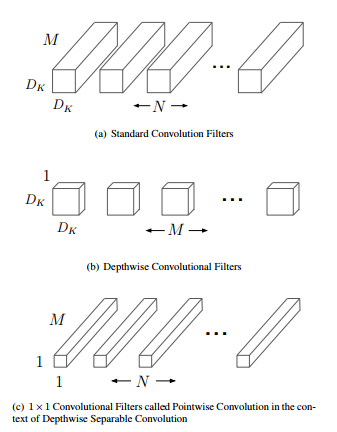
\includegraphics[width=0.7\textwidth]{convolucionesMobilenet}%
          \caption[División filtros convolucionales]{Los filtros convolucionales normales son divididos en los filtros profundos y los puntuales.}%
          \label{figconvolucionesMobilenet}%
        \end{center}%
  	\end{center}%
\end{figure}%

El uso de estos tipos de filtros de forma paralela, más el uso de filtros de normalización y pooling, es lo que usa Mobilenet para ejecutarse de forma rápida y utilizando la menor cantidad de memoria posible.

\section{Data Augmentation}

	El Data Augmentation es una técnica que busca ampliar el conjunto de datos de entrenamiento, aplicando unas serie de transformaciones sobre las imágenes iniciales \cite{NIPS2012_4824}.
	
En las imágenes de entrenamiento se aplican una serie de técnicas como son la rotación, recortes, incremento del brillo, cambio de la gama de colores  entre otras, para conseguir nuevas imágenes que usar para el entrenamiento del clasificador.

Esta técnica nos permite ampliar nuestro conjunto de datos sin tener almacenadas estas imágenes extras a cambio de un procesamiento extra a la hora de entrenar.

Para evitar el sobreajuste del modelo, ya que estas imágenes creadas están muy interrelacionadas entre si, se ejecutan las transformaciones con una probabilidad, disminuyendo así el número de imágenes artificiales.


\section{Web Semántica}

La Web semántica es una Web extendida desarrollada bajo los estándares W3C (World Wide Web Consortium). Esta Web extendida aplica metadatos a la información que recoge para que los usuarios puedan encontrar respuestas de una manera más rápida y sencilla gracias a esta información adicional \cite{webSemantica}.

Estos metadatos son los que otorgan más semántica a la Web y permiten obtener soluciones a problemas habituales gracias al uso de una arquitectura común para toda la información. 

Por ejemplo, en este proyecto, esta tecnología ha permitido automatizar todo el proceso de recogida de información de las diferentes especies de setas de una manera rápida y eficaz.

\subsection{¿Para qué sirve?}

A la Web actual que todos conocemos le podemos atribuir dos problemas que han surgido del enorme crecimiento que ha tenido. Estos problemas son una sobrecarga de información, mucha de la información esta repetida en diferentes lugares siendo la misma, y que la información no se muestra bajo una estructura común, sino de una forma heterogénea.

La web semántica busca solucionar estos problemas delegándolos en el software, este software es capaz de procesar su contenido, combinarlo y realizar deducciones lógicas para solucionar problemas habituales.

\subsection{¿Cómo funciona?}

El funcionamiento de la web semántica se basa esencialmente en RDF, SPARQL y OWL, mecanismos que permiten convertir la estructura de la Web para que se adecue al funcionamiento de una Web Semántica.
\begin{itemize}
	\item{RDF}: RDF permite introducir metadatos descriptivos en los distintos tipos de información.
	\item{SPARQL}: Es el lenguaje de consultas que nos permite realizar búsquedas sobre la información que contiene estos metadatos.
	\item{OWL}:OWL permite crear vocabularios para asociar los diferentes recursos.
\end{itemize}

El uso conjunto de estos mecanismos es el que nos permite razonar sobre los datos de la Web.

\section{Web Scraping}

La herramienta del Web Scraping es una herramienta para extraer información o datos de páginas web de una manera rápida, eficiente y automatizada. La información extraída se presenta de una forma más estructurada y fácil de usar \cite{webScraping}.

Los programas para realizar Web Scraping se pueden programar en diferentes lenguajes de programación, los más populares son Java, Python, Ruby y Node. Además existen diversos programas para realizar estas acciones mediante un interfaz gráfico.

Aproximadamente el 70\% de la información publicada en Internet esta en formato PDF, un formato no estructurado y difícil de manejar. Sin embargo, las páginas web si que tienen un formato estructurado ya que están programadas en código HTML, pero aun así no están presentadas de una manera totalmente reutilizable ya que no todas siguen el mismo esquema.

La técnica más extendida de Web Scraping es analizar la estructura del código HTML propio de una página web para poder extraer la información buscada. Por ejemplo, extraer todos los atributos text de los label <p> que se encuentren en una determinada página Web.


\section{Clave Dicotómica}

Las claves dicotómicas son herramientas que periten identificar organismos. Las claves pueden determinar animales, plantas, hongos,moneras, protistas o cualquier otro ser vivo. Las claves pueden alcanzar diferentes profundidades identificando el género, especie, familia, entre otros.

La clave dicotómica se basa en ir mostrando al usuario diferentes dilemas (afirmaciones contrapuestas) entre los que deberá ir eligiendo el que más se adecue al organismo a identificar hasta alcanzar la categoría taxonómica\footnote{Grupos en los que se clasifican los seres vivos.} deseada. Estas afirmaciones están enumeradas a lo largo de la clave.

\subsection{¿Cómo usar una clave?}

Usar una clave consiste simplemente en leer los diferentes dilemas y optar solamente por uno de ellos. El dilema elegido no volverá a aparecer en el desarrollo de la clave \cite{claveDicotomica}.



































































\capitulo{4}{Técnicas y herramientas}

Esta parte de la memoria tiene como objetivo presentar las técnicas metodológicas y las herramientas de desarrollo que se han utilizado para llevar a cabo el proyecto. Si se han estudiado diferentes alternativas de metodologías, herramientas, bibliotecas se puede hacer un resumen de los aspectos más destacados de cada alternativa, incluyendo comparativas entre las distintas opciones y una justificación de las elecciones realizadas. 
No se pretende que este apartado se convierta en un capítulo de un libro dedicado a cada una de las alternativas, sino comentar los aspectos más destacados de cada opción, con un repaso somero a los fundamentos esenciales y referencias bibliográficas para que el lector pueda ampliar su conocimiento sobre el tema.



\capitulo{5}{Aspectos relevantes del desarrollo del proyecto}

%Este apartado pretende recoger los aspectos más interesantes del desarrollo del proyecto, comentados por los autores del mismo.
%Debe incluir desde la exposición del ciclo de vida utilizado, hasta los detalles de mayor relevancia de las fases de análisis, diseño e implementación.
%Se busca que no sea una mera operación de copiar y pegar diagramas y extractos del código fuente, sino que realmente se justifiquen los caminos de solución que se han tomado, especialmente aquellos que no sean triviales.
%Puede ser el lugar más adecuado para documentar los aspectos más interesantes del diseño y de la implementación, con un mayor hincapié en aspectos tales como el tipo de arquitectura elegido, los índices de las tablas de la base de datos, normalización y desnormalización, distribución en ficheros3, reglas de negocio dentro de las bases de datos (EDVHV GH GDWRV DFWLYDV), aspectos de desarrollo relacionados con el WWW...
%Este apartado, debe convertirse en el resumen de la experiencia práctica del proyecto, y por sí mismo justifica que la memoria se convierta en un documento útil, fuente de referencia para los autores, los tutores y futuros alumnos.

En este apartado se va a recoger el ciclo de vida del proyecto, detallando los aspectos más relevantes que se han tratado y como se han resuelto las diferentes  dificultades encontradas a lo largo de su desarrollo.

Se irán presentando diferentes secciones que concuerdan con el orden cronológico seguido en el proyecto y muestran la justificación de las decisiones tomadas.

\section{Propuesta del proyecto}

La propuesta de este proyecto consistía en crear una aplicación Android para el reconocimiento de setas que se dividía en las siguientes 3 tareas principales:

\begin{itemize}
	\item{Clasificador de imágenes:} La tarea principal pedida para realizar este proyecto era la de construir un clasificador visual de imágenes que a través de la foto realizada a una seta nos devolviera un listado de las especies más probables.
	\item{Web Semántica:} Conseguir información a través de una web semántica para documentar las especies de setas incluidas en el clasificador.
	\item{Clave dicotómica:} Incorporar una clave dicotómica que reforzara la tarea del clasificador para el reconocimiento de la especie.
\end{itemize}

Ante estas tareas se empezó a investigar que alternativas había para construir una aplicación que fuera lo suficientemente precisa y de fácil uso para el usuario. Se barajaron las siguientes posibilidades:

\begin{itemize}
	\item{Incorporar sólo un clasificador visual:} Si sólo se implementaba un clasificador visual en la aplicación, esta sería muy fácil de usar pero sería poco precisa ya que clasificar la especie de una seta por una única foto es una tarea casi imposible. 
	\item{Clasificador visual con elección manual entre las candidatas:} La idea de esta propuesta es la de mostrar al usuario un listado con las cinco especies más probables clasificadas para esa foto y que este las pueda comparar mediante fotografías proporcionadas por la aplicación de esas especies con su foto. Esta propuesta puede ser un poco más fiable pero depende de los conocimientos del usuario y la hace más compleja.
	\item{Clave dicotómica única:} Incluir una clave dicotómica aislada del clasificador podía proporcionar una gran fiabilidad pero suelen ser claves de difícil uso para el usuario.
	\item{Clave dicotómica más el clasificador:} Esta propuesta consistía en filtrar las preguntas de la clave dicotómica en base a los resultados obtenidos por el clasificador de imágenes.
\end{itemize}

Con estas propuestas en mente se empezó a estudiar como se podía implementar el clasificador de imágenes y como podíamos implementar las diferentes propuestas en base a lo que se iba desarrollando.

\section{¿Cómo implementar el clasificador?}

Se decidió empezar por la tarea de generar el clasificador de imágenes ya que era la tarea más complicada de realizar y de la que dependían las demás tareas. En la asignatura de minería de datos ya había adquirido conocimientos sobre como entrenar y usar clasificadores de imágenes pero ahora surgía la duda de como hacer esto mismo pero en una plataforma nueva para mí que era Android. En las primeras reuniones del proyecto los profesores me propusieron las siguientes posibilidades para realizarlo:

\begin{itemize}
	\item Entrenar un clasificador de imágenes desde cero que se ejecutara en un servidor Web y mostrara los resultados en el teléfono móvil.
	\item Seguir la propuesta anterior pero reentrenando una red neuronal en vez de entrenar un modelo desde cero.
	\item Reentrenar los nuevos modelos Mobilenet mediante Tensorflow, lo que nos permitiría ejecutar los clasificadores en el propio dispositivo móvil.
\end{itemize}

Elegí empezar por estudiar la tercera propuesta y ver si era posible ejecutar los modelos en el propio teléfono móvil. Esta propuesta tiene la ventaja de que el usuario no necesita estar conectado a un servidor Web, característica importante si pensamos que esta aplicación se usaría en zonas con poca cobertura.

La preocupación principal era saber si los modelos se iban a poder ejecutar en el propio móvil de una manera rápida, ya que es un proceso costoso, y que nos proporcionara los resultados deseados. Después de estudiar la tecnología Tensorflow y cómo implementarla en una aplicación Android probé varios varios modelos preentrenados de prueba que proporcionan en los ejemplos de Tensorflow\footnote{\url{https://github.com/tensorflow/tensorflow/tree/master/tensorflow/examples/android}} y vi que la aplicación se ejecutaba correctamente en diferentes modelos de móvil simulados y en mi propio teléfono.

Esta etapa del proyecto me permitió empezar a familiarizarme con el entorno de programación Android Studio y con las librerías de Tensorflow.

Después de realizar pruebas con modelos preentrenados y ejemplos empecé a estudiar como poder entrenar mi propio modelo de Mobilenet o Inception, con nuestro repositorio de imágenes de setas, para que diferenciara entre las diferentes especies. La solución la encontré en el mismo repositorio de Github\footnote{\url{https://github.com/tensorflow/tensorflow/tree/master/tensorflow/examples/image_retraining}} de Tensoflow en el que proporcionan un script en python ("retrain.py") para reentrenar ambos modelos pudiendo modificar gran variedad de parámetros y ajustes para crear un modelo personalizado.

Gracias a estos scripts y a los ejemplos encontrados de Tensorflow en Android conseguí reentrenar los primeros modelos y clasificar las primeras imágenes en el propio móvil.

Las imágenes usadas para entrenar los modelos se sacaron de los repositorios Imagenet y Enciclopedia of Life, recopilando aproximadamente entre 30 y 80 fotos por cada especie de seta. En total se han usado 9400 fotografías para reentrenar el clasificador completo divididas en 171 especies de setas.

Las primeras pruebas se ejecutaron con un modelo Mobilenet v1-224 reentrenado, que diferenciaba 118 especies de setas, en un teléfono móvil Samsung galaxy S5. La aplicación lograba ejecutarse fluidamente y se consiguió una precisión (61,5\%)\ref{figMobilenet1} en la validación cruzada con 4000 pasos de reentrenamiento:

\begin{figure}[h]
    \begin{center}%
        \begin{center}%
          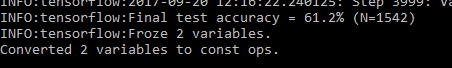
\includegraphics[width=1\textwidth]{mobilenet1}%
          \caption{Mobilenet v1-224, 4000 steps, 118 especies.}%
          \label{figMobilenet1}%
        \end{center}%
  	\end{center}%
\end{figure}%

Aunque la precisión de estos modelos no sea relativamente alta, nos basta con que la especie correcta se encuentre entre los cinco primeros resultados del clasificador, ya que este clasificador se complementará con la clave dicotómica.

\section{¿Qué modelo de clasificador usar?}

Para elegir el modelo a usar se tuvieron que tener en cuenta diferentes factores como el peso del modelo, su carga de computo y su precisión. En teoría el modelo Inception es más preciso que el Mobilenet pero requiere mayor capacidad de computo y espacio de almacenamiento, recursos que son limitados en los teléfonos móviles.

Para Mobilenet contábamos con los modelos mostrados en la figura \ref{figComparativaMobilenet} mientras que de Inception solo podía reentrenar el modelo Inception v3.

\begin{figure}[h]
    \begin{center}%
        \begin{center}%
          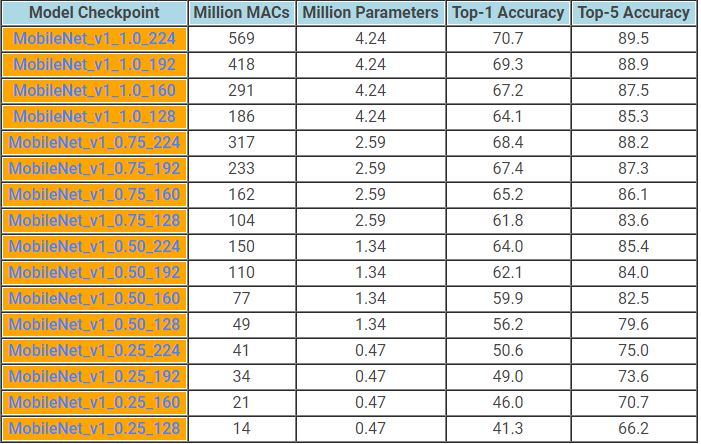
\includegraphics[width=1\textwidth]{comparativaMobilenet}%
          \caption{Comparativa modelos Mobilenet}%
          \label{figComparativaMobilenet.}%
        \end{center}%
  	\end{center}%
\end{figure}%
\newpage
Se realizaron pruebas con los diferentes modelos y al final opte por usar el modelo Mobilenet v1 224 ya que se ejecutaba de forma suficientemente fluida y proporciona una precision superior a los demás modelos Mobilenet. 

Respecto al modelo Inception su peso era de 75 Megabytes en contra de los 17 Megabytes que ocupaba el modelo Mobilenet y los resultados obtenidos \ref{figInception1} en validación cruzada eran parecidos entrenados en las mismas condiciones. 

%https://opensource.googleblog.com/2017/06/mobilenets-open-source-models-for.html
\begin{figure}[h]
    \begin{center}%
        \begin{center}%
          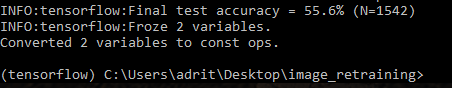
\includegraphics[width=1\textwidth]{inception1}%
          \caption{Inception v3, 4000 steps, 118 especies.}%
          \label{figInception1}%
        \end{center}%
  	\end{center}%
\end{figure}%

Una vez elegido el modelo se procedió a escalar el modelo aumentando el número de especies a diferenciar, pasando de clasificar 118 especies a un total de 171. Este aumento provoco un ligero descenso en la precisión del clasificador que se solvento aplicando técnicas de Data augmentation a la hora de entrenar el modelo. La precisión obtenida final fue de un 59,4\% \ref{figMobilenet2} en validación cruzada de media entre todas las categorías de especies de setas.

Se probó a aumentar el número de pasos de entrenamiento pero esto no provocaba un ascenso de la precisión sino que se mantenía constante y provocaba el riesgo de que se sobre entrenara el modelo por lo que se decidio dejar el parámetro en 4000 pasos.

El tiempo necesario para entrenar este modelos con un procesador i7 4790, fue de 5 horas 55 minutos.

\begin{figure}[h]
    \begin{center}%
        \begin{center}%
          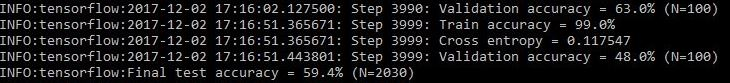
\includegraphics[width=1\textwidth]{mobilenet2}%
          \caption{Mobilenet v1-224, 4000 steps, 172 especies, con data augmentation.}%
          \label{figMobilenet2}%
        \end{center}%
  	\end{center}%
\end{figure}%

\section{Web Semántica}

La siguiente tarea que se decidió afrontar después de implementar el clasificador de imágenes fue la parte de Web semántica. En esta tarea había que recopilar información de las diferentes especies de setas, de alguna Web semántica, con el objetivo de crear fichas para cada especie que pudiera consultar el usuario en cualquier momento.

La principal dificultad que se encontró en este apartado y que determino el uso de la DBpedia como Web semántica, fue encontrar un repositorio que contuviera información suficiente de todas las especies sin excepción.El alto número de especies que podía clasificar la aplicación dificultaba esta tarea. Este requisito era necesario para automatizar la extracción de datos y que todas las especies tuvieran su ficha de información.

La DBpedia era la única que recopilaba información suficiente de todas las especies al completo y nos proporcionaba la información mínima deseada como era una descripción de la especie y la comestibilidad de esta.

Otra opción que se contemplo fue la de usar web scraping en vez de consultas a una web semántica, pero esta opción se descarto ya que no se logro encontrar un repositorio con todas la especies y que contuviera más información que la que proporcionaba por la DBpedia.

Gracias al lenguaje de consultas SparQL y la librería Apache Jena para Java se implemento un programa en Windows que realizaba consultas a la DBpedia y nos devolvía la información necesaria.

El siguiente problema a afrontar era como almacenar y transferir esta información a la aplicación Android. Después de estudiar diferentes bases de datos se opto por usar la base de datos SQLite. Esta base de datos tiene soporte tanto para Android como para Windows por lo que es fácil exportar los datos de una plataforma a otra. Además no requiere de configuración de usuarios ni conexiones lo que simplifica su uso. Aunque proporcione una funcionalidad básica, esta base de datos nos permitía almacenar nuestra información y cumplía con los requisitos de la aplicación.

Para mostrar imágenes comparativas de las especies se usaron una parte de las imágenes ya recopiladas, que se habían usado para entrenar el clasificador. Estas imágenes se formatearon en una resolución menor que la original para ahorrar espacio en la aplicación. Estas imágenes se almacenaron dentro de la propia estructura de la aplicación Android.

Una vez recopilada la información de las diferentes especies, la aplicación era capaz de clasificar las cinco especies más probables respecto a la imagen de la seta introducida, mostrar imágenes comparativas de las especies y mostrar información de cada especie.

De cara a la internacionalización de la aplicación se implemento un método que tradujera automáticamente mediante el traductor de Google la información de la DBpedia en caso de no estar disponible en el idioma deseado. Por ejemplo, había veces que la información no se encontraba disponible en Español por lo que se traducía desde la versión en inglés.

\section{Clave dicotómica}

El último apartado a tratar era el de implementar una clave dicotómica que nos permitiera diferenciar entre todos los géneros contenidos en el clasificador. Esta tarea tenia las dos siguientes dificultades:

\begin{itemize}
	\item Conseguir una clave dicotómica que discriminara entre todos los géneros de especies del clasificador.
	\item Estructurar esa clave dicotómica de una forma que se pudiera manejar para implementarse en la aplicación Android.
\end{itemize}

Después de buscar en diferentes páginas web, se encontró una (\url{http://www.avelinosetas.info/claves.php}) que contenía una serie de claves dicotómicas para diferentes especies y una clave que discriminaba entre 108 géneros de setas. De las claves encontradas fue la que más géneros contemplaba. Para que los géneros de la clave y del clasificador coincidieran se recopilaron imágenes de las especies que no se contemplaban en el clasificador para reentrenarlo y que pudiera discriminar entre 171 especies distintas.

Esta solución tiene la limitación de que el número de setas discriminado por el clasificador no es el mismo que el de la clave dicotómica.

Para extraer las claves de la página Web se desarrollo un programa en Java que mediante técnicas de Web Scraping extrajera las claves dicotómicas y las almacenar en estructuras de datos que nos permitieran usarlas para nuestra aplicación Android.

Además de la clave general de géneros, se extrajeron las claves dicotómicas disponibles para diferenciar entre especies concretas dentro de un mismo género.

Esta tarea se pudo automatizar mediante la herramienta Jaunt para Java revisando el código html de la página Web.











\capitulo{6}{Trabajos relacionados}

%Este apartado sería parecido a un estado del arte de una tesis o tesina. En un trabajo final grado no parece obligada su presencia, aunque se puede dejar a juicio del tutor el incluir un pequeño resumen comentado de los trabajos y proyectos ya realizados en el campo del proyecto en curso. 

\section{Otros proyectos}

Este proyecto partía del trabajo de Máster \textit{Reconocimiento de setas mediante visión artificial y sistema experto IberoSetas 2.0} realizado por Iñaki Arroyo Nebreda en el año 2014. Aunque el trabajo actual contemplaba objetivos parecidos, decidí empezar mi trabajo desde cero ya que se han usado tecnologías diferentes y se ha generado la aplicación desde una perspectiva diferente \cite{iberosetas}.

Para la parte del clasificador, en el trabajo anterior se creo un clasificador de imágenes en un servidor remoto al que debía conectarse la aplicación móvil. Para ello se tuvieron que preprocesar las imágenes para extraer sus características mediante técnicas como el \textit{Bag of words} y a partir de esta información entrenar un clasificador como pudieran ser el J48 o el KNN (\textit{k-nearest neighbor}).

En nuestro caso se han usado las recientes versiones de redes neuronales de Mobilenet e Inception desarrolladas por Google. Estos modelos realizan la extracción de características y están diseñados para ejecutarse de manera eficiente en las arquitecturas de los teléfonos móviles.

Gracias a estos avances tecnológicos se han conseguido clasificar 171 especies respecto a las 10 que clasificaba el trabajo anterior, realizando la tarea en el propio dispositivo móvil sin necesidad de una conexión a Internet a un servido externo.

La parte de la clave dicotómica en el trabajo anterior se realizó codificando una clave de 10 géneros sobre un formato xml. En este trabajo se han realizado técnicas de Web Scraping que nos han permitido extraer diferentes claves que cubren un mayor número de géneros y especies, codificandolas directamente en estructuras de datos Java.

La parte de web semántica se ha realizado de igual forma aplicando consultas sobre la DBpedia.

\section{Aplicaciones relacionadas}

Se ha encontrado una aplicación, que se lanzó a mediados de Octubre de 2017, en la que se puede clasificar setas a través de imágenes de manera similar a lo propuesto en este proyecto. La aplicación se puede encontrar en el siguiente link \url{https://play.google.com/store/apps/details?id=com.pingou.champignouf&hl=es}

La principal diferencia de esta aplicación es que necesitas conexión a Internet para clasificar la imagen de la seta, a diferencia de nuestra aplicación, que se clasifica en el propio móvil.

No se han encontrado más aplicaciones que realicen este tipo de clasificación de setas en los dispositivos móviles.

Podemos encontrar una comparativa entre las dos aplicaciones en la siguiente tabla:
\clearpage
\tablaSmall{Ubusetas 1.0 vs Identificador Setas 2.17}{l c c}{comparativaAplicaciones}
{ \multicolumn{1}{l}{Características} & Ubusetas 1.0 & Identificador Setas 2.17 \\}{ 
Instalación sencilla & Sí & Sí  \\
Requiere conexión a Internet & No & Sí \\
Procesamiento en local & Sí & No \\
Información comestibilidad & Sí & Sí \\
Descripción seta & Sí & Sí \\
Velocidad clasificación & Instantánea & Depende del servidor \\
Mercado setas & No & Sí \\
Localización GPS & No & Sí \\
} 
\capitulo{7}{Conclusiones y Líneas de trabajo futuras}

%Todo proyecto debe incluir las conclusiones que se derivan de su desarrollo. Éstas pueden ser de diferente índole, dependiendo de la tipología del proyecto, pero normalmente van a estar presentes un conjunto de conclusiones relacionadas con los resultados del proyecto y un conjunto de conclusiones técnicas. 
%Además, resulta muy útil realizar un informe crítico indicando cómo se puede mejorar el proyecto, o cómo se puede continuar trabajando en la línea del proyecto realizado. 


\section{Conclusiones}

Respecto a los requisitos del proyecto, creo que se han cumplido ofreciendo un clasificador de especies que puede servir de ayuda en la práctica de la micología, de una manera rápida y accesible para los usuarios, apoyándose en las diferentes claves dicotómicas e información disponible de manera local.

A nivel personal, he adquirido nuevos conocimientos relacionados con la minería de datos, clasificación de imágenes, Web scraping, web semántica, planificación, uso de Latex y  el desarrollo en Android, entre otros, permitiéndome manejarme con mayor soltura en estos campos.

Respecto a las dificultades encontradas, algunas han surgido por intentar abarcar una gran cantidad de especies, lo que ha significado tener que encontrar un gran número de imágenes y de información de setas, además de dificultar la tarea de implementar una clave dicotómica que contuviese todos los géneros clasificados.

La escasez de imágenes de algunas especies se ha resuelto gracias a aplicar técnicas de data augmentation así como poder usar diferentes claves dicotómicas gracias a la aplicación de web scraping. El problema de automatizar la recolección de las claves dicotómicas es que no todas se presentaban de manera uniforme en la página web y este hecho ha dado problemas para poder recuperarlas, teniendo que suprimir algunas de estas claves disponibles. Aún así, considero que se han conseguido suficientes claves para las especies disponibles.

En general estoy satisfecho con el trabajo realizado y con las aplicaciones propuestas.

\section{Líneas de trabajo futuras}

A continuación se muestra un listado de aplicaciones y mejoras que se podrían incorporar en futuros proyectos:

\begin{itemize}
	\item Implementar un sistema de localización en el que el usuario pueda compartir donde ha encontrado una especie de seta en concreto.
	\item Implementar nuevas bases de datos que suministren información de las diferentes setas además de la DBpedia.
	\item Expandir el clasificador aumentando el número de especies o imágenes
	\item Implementar un sistema de aprendizaje en el que la aplicación pregunte al usuario sobre una seta, y este tenga que adivinar la especie.
	\item Generar un sistema en el que el usuario se pueda registrar y llevar un listado de las setas que ha ido clasificando a lo largo de su uso con la aplicación.
	\item Almacenar la información recopilada por los usuarios en un servidor para usarla en otras aplicaciones como podría ser, indicar en que zonas hay determinadas especies y en que momento se han encontrado.
	\item Generar un mercado virtual en el que los usuarios puedan vender y comprar diferentes tipos de setas.
\end{itemize}



\bibliographystyle{plain}
\bibliography{bibliografia}

\end{document}
